% \documentclass[handout]{beamer}
% \documentclass[presentation]{beamer}
\documentclass[8pt, aspectratio=169]{beamer} % Wide presentation format
% \documentclass[8pt]{beamer}       % Narrow presentation format

\usecolortheme{Blue}
 
\usepackage[utf8]{inputenc}
\usepackage[UKenglish]{babel}
\usepackage{booktabs}
\usepackage{caption}
\usepackage{subcaption}
\usepackage{graphicx}
\usepackage{amsmath}
\usepackage{amsfonts}
\usepackage{amssymb}
\usepackage{epstopdf}
%\usepackage{enumitem} %Comment out enumitem if you want round ("default") bullet points
%\useinnertheme{rectangles} % Uncomment this (and comment out enumitem) if you want to use different bullet points
\usepackage{hyperref}
\usepackage[style=numeric]{biblatex}
\usepackage{listings}


% Set label of itemize lists - default are circle bullets
%\setlist[itemize]{label=-}


\addbibresource{references.bib}


% complying UK date format, i.e. 1 January 2001
\usepackage{datetime}
\let\dateUKenglish\relax
\newdateformat{dateUKenglish}{\THEDAY~\monthname[\THEMONTH] \THEYEAR}

%Define new command for hyperlinks
\newcommand{\link}[2]{{\color{blue}\href{#2}{#1}}}

% Add your logo here
\logo{%
    
\includegraphics[height=1cm,keepaspectratio]{assets/placeholder_logo.png}~%
    \vspace{210pt}
}


% -----------------------------------------------------------------------------




%Information to be included in the title page:

\title{Presentation Title}

\subtitle{Subtitle or Author}

\author{Author or Contact}

\date{\today}


\begin{document}
 
\frame{\titlepage}

%-------------------------------------------------------------------

\begin{frame}{Overview}
    \begin{itemize}
        \item Bullet 1
        \vspace{10pt}
        \item Bullet 2
        \vspace{10pt}
        \item Bullet 3
        \vspace{10pt}
        \item Bullet 4
        \vspace{10pt}
        \item Bullet 5
        \vspace{10pt}
        \item Bullet 6
    \end{itemize}
\end{frame}

\section{Section A}
\begin{frame}{Slide Title}
    \begin{figure}
      \centering
      \begin{minipage}[b]{0.3\textwidth}
        \centering
        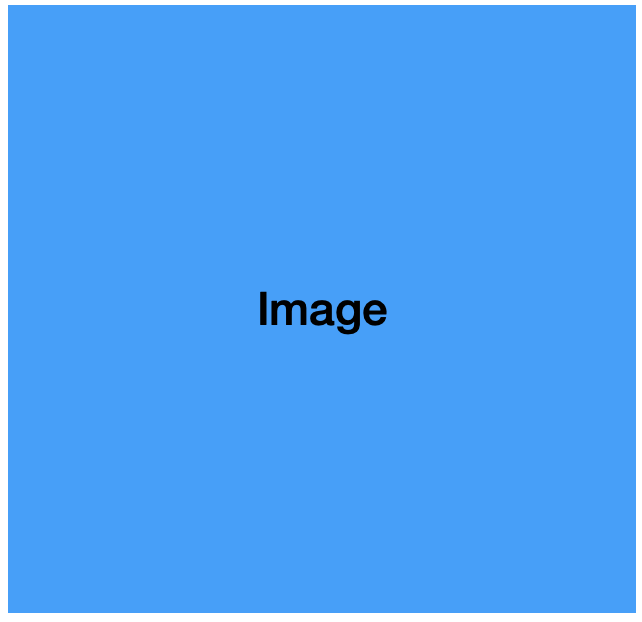
\includegraphics[width=0.9\textwidth]{assets/placeholder_img.png}
      \end{minipage}
      \hfill
      \begin{minipage}[b]{0.3\textwidth}
        \centering
        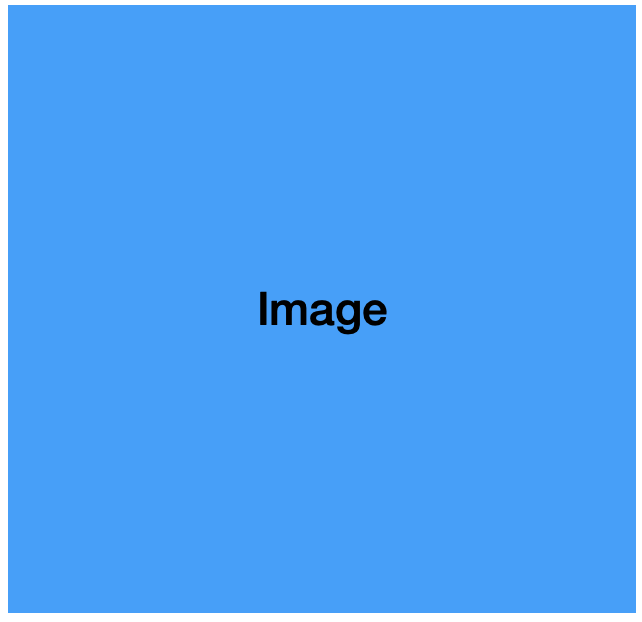
\includegraphics[width=0.9\textwidth]{assets/placeholder_img.png}
      \end{minipage}
      \hfill
      % \hspace{20pt}
      \begin{minipage}[b]{0.35\textwidth}
        \begin{itemize}
        \item Bullet with citation \cite{Author1Title}
        \item Bullet
        \item Bullet
        \item Bullet
    \end{itemize}
    \vspace{20pt}
      \end{minipage}
    \end{figure}
\end{frame}

\begin{frame}{Title}
    \begin{figure}[!tbp]
      \centering
      \begin{minipage}[b]{0.4\textwidth}
        \centering
        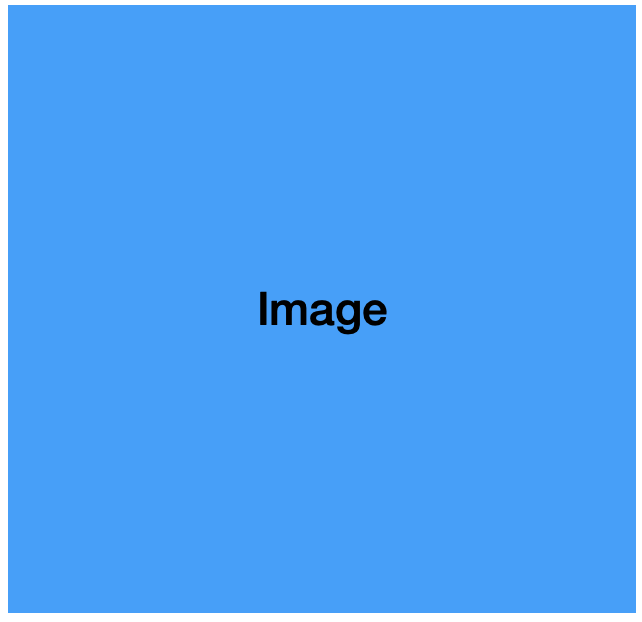
\includegraphics[width=0.8\textwidth]{assets/placeholder_img.png}
      \end{minipage}
      \hspace{20pt}
      \begin{minipage}[b]{0.4\textwidth}
        \centering
        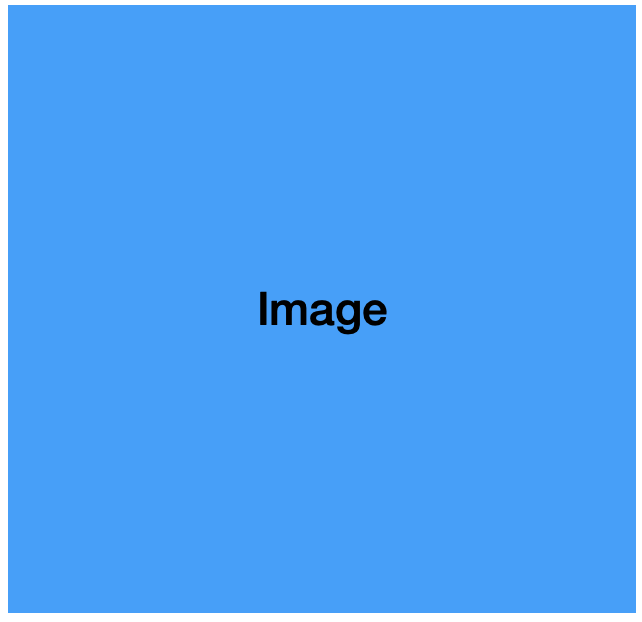
\includegraphics[width=0.8\textwidth]{assets/placeholder_img.png}
      \end{minipage}
    \end{figure}
\end{frame}


\begin{frame}{Title}

    \begin{itemize}
        \item Bullet
        \vspace{15pt}
        \item Bullet...
        \item[ ] ... Bullet \footnote{footnote}  ...
        \item[ ] \hspace{10pt} ... Bullet
        \vspace{15pt}
        \item Bullet
        \item Bullet
    \end{itemize}
\end{frame}


\section{Section B}

\begin{frame}{Title}
    \vspace{10pt}
    \begin{table}
    \centering
    % \scriptsize
    \begin{tabular}{lccccccc} 
        \toprule
        & Column 1 & Column 2 & Column 3 & Column 4 & Column 5 & Column 6 \\ 
        \midrule
        Row 1 & 1.0 ± 0.5  & 1.0 ± 0.5 & 1.0 ± 0.5 & 1.0 ± 0.5 & \textbf{1.0 ± 0.5} & 1.0 ± 0.5 \\
        Row 2 & 1.0 ± 0.5  & 1.0 ± 0.5 & 1.0 ± 0.5 & 1.0 ± 0.5 & \textbf{1.0 ± 0.5} & 1.0 ± 0.5 \\
        Row 3 & 1.0 ± 0.5  & 1.0 ± 0.5 & 1.0 ± 0.5 & 1.0 ± 0.5 & \textbf{1.0 ± 0.5} & 1.0 ± 0.5 \\
        Row 4 & 1.0 ± 0.5  & 1.0 ± 0.5 & 1.0 ± 0.5 & 1.0 ± 0.5 & \textbf{1.0 ± 0.5} & 1.0 ± 0.5 \\
        Row 5 & 1.0 ± 0.5  & 1.0 ± 0.5 & 1.0 ± 0.5 & 1.0 ± 0.5 & \textbf{1.0 ± 0.5} & 1.0 ± 0.5 \\
        \midrule
        Row 6 & 1.0 ± 0.5  & 1.0 ± 0.5 & 1.0 ± 0.5 & 1.0 ± 0.5 & \textbf{1.0 ± 0.5} & 1.0 ± 0.5 \\
        Row 7 & 1.0 ± 0.5  & 1.0 ± 0.5 & 1.0 ± 0.5 & 1.0 ± 0.5 & \textbf{1.0 ± 0.5} & 1.0 ± 0.5 \\
        Row 8 & 1.0 ± 0.5  & 1.0 ± 0.5 & 1.0 ± 0.5 & 1.0 ± 0.5 & \textbf{1.0 ± 0.5} & 1.0 ± 0.5 \\
        Row 9 & 1.0 ± 0.5  & 1.0 ± 0.5 & 1.0 ± 0.5 & 1.0 ± 0.5 & \textbf{1.0 ± 0.5} & 1.0 ± 0.5 \\
        Row 10 & 1.0 ± 0.5  & 1.0 ± 0.5 & 1.0 ± 0.5 & 1.0 ± 0.5 & \textbf{1.0 ± 0.5} & 1.0 ± 0.5 \\
        \bottomrule
    \end{tabular}
    \caption{Table caption}
\end{table}
\end{frame}


\begin{frame}{Title}
    \begin{enumerate}
        \pause
        \item Bullet
            \begin{enumerate}
                \pause
                \item[1.1] Bullet
                \pause
                \item[1.2] Bullet
                \pause
                \item[1.3] Bullet
            \end{enumerate}
        \pause
        \item Bullet
            \begin{enumerate}
                \pause
                \item[2.1] Bullet
                \pause
                \item[2.2] Bullet
            \end{enumerate}
        \pause
        \item Bullet
            \begin{enumerate}
                \pause
                \item[3.1] Bullet
                \pause
                \item[3.2] Bullet
            \end{enumerate}
        \end{enumerate}
\end{frame}

%-------------------------------------------------------------------
\section{References}

\begin{frame}[allowframebreaks]{References}
    \printbibliography[heading=none]
\end{frame}

\end{document}

